\section{Evaluation}
\label{sec:eval}

% Set listing style for table
\lstset{
	frame=none,
    aboveskip=0pt,
    belowskip=0pt,
    basicstyle=\tiny\ttfamily,
}
\begin{table*}\scriptsize
\caption{Complementary code examples}
\label{tab:compl-examples}

\setlength{\tabcolsep}{0.01\textwidth}
\begin{tabular}{@{}p{0.49\textwidth}p{0.49\textwidth}@{}}
\toprule
Query Code Snippet & Recommended Related Code \\
\midrule



\begin{lstlisting}
public static boolean unpackZip(String path, String zipname, String targetDirectory) {
	InputStream is;
	ZipInputStream zis;
	try {
		String filename;
		is = new FileInputStream(path + zipname);
		zis = new ZipInputStream(new BufferedInputStream(is));
		ZipEntry ze;
		byte[] buffer = new byte[1024];
		int count;

		while ((ze = zis.getNextEntry()) != null) {
			filename = ze.getName();

			if (ze.isDirectory()) {
				File fmd = new File(targetDirectory + filename);
				fmd.mkdirs();
				continue;
			}

			FileOutputStream fout = new FileOutputStream(targetDirectory + filename);

			while ((count = zis.read(buffer)) != -1) {
				fout.write(buffer, 0, count);
			}

			fout.close();
			zis.closeEntry();
		}

		zis.close();
	} catch (IOException e) {
		e.printStackTrace();
		return false;
	}

	return true;
}
\end{lstlisting}


&
\begin{lstlisting}
public static void zip(String baseFolder, List<File> files, String zipFile) {
	try  {
		BufferedInputStream origin = null;
		FileOutputStream dest = new FileOutputStream(zipFile);

		ZipOutputStream out = new ZipOutputStream(new BufferedOutputStream(dest));
		byte data[] = new byte[BUFFER];

		for (File file : files) {
			FileInputStream fi = new FileInputStream(file);
			origin = new BufferedInputStream(fi, BUFFER);
			String relativeFileName = file.getAbsolutePath().replace(baseFolder + File.separator , """");
			ZipEntry entry = new ZipEntry(relativeFileName);
			out.putNextEntry(entry);
			int count;
			while ((count = origin.read(data, 0, BUFFER)) != -1) {
				out.write(data, 0, count);
			}
			origin.close();
		}

		out.close();
	} catch(Exception e) {
		e.printStackTrace();
	}

}
\end{lstlisting}
\vspace*{1em}
\explanation{
    \emph{Example A: Complementary method}
    \begin{itemize}
        \item The query snippet implements unzip a folder in Java.
        \item The recommended related method implements zip a folder. These two methods can function independently, but often implemented together to get a stronger ability for folder manipulation.
    \end{itemize}
}

\\

\bottomrule

\begin{lstlisting}
public static byte[] encrypt(final SecretKeySpec key, final byte[] iv, final byte[] message)
throws GeneralSecurityException {
	final Cipher cipher = Cipher.getInstance(AES_MODE);
	IvParameterSpec ivSpec = new IvParameterSpec(iv);
	cipher.init(Cipher.ENCRYPT_MODE, key, ivSpec);
	byte[] cipherText = cipher.doFinal(message);

	log(""cipherText"", cipherText);

	return cipherText;
}
\end{lstlisting}


&
\begin{lstlisting}
public static byte[] decrypt(final SecretKeySpec key, final byte[] iv, final byte[] decodedCipherText)
throws GeneralSecurityException {
	final Cipher cipher = Cipher.getInstance(AES_MODE);
	IvParameterSpec ivSpec = new IvParameterSpec(iv);
	cipher.init(Cipher.DECRYPT_MODE, key, ivSpec);
	byte[] decryptedBytes = cipher.doFinal(decodedCipherText);

	log(""decryptedBytes"", decryptedBytes);

	return decryptedBytes;
}
\end{lstlisting}

\vspace*{1em}
\explanation{
	\emph{Example B: Complementary method}
	\begin{itemize}
		\item The query snippet implements \texttt{encrypt} functionality for an byte array.
		\item The recommended related method decrypts a decoded byte array. 
	\end{itemize}
}

\\

\bottomrule

\begin{lstlisting}
@Override
public void onCreate(Bundle savedInstanceState) {
	super.onCreate(savedInstanceState);
	setContentView(R.layout.main);
	preferred = (TextView)findViewById(R.id.preferred);
	orientation = (TextView)findViewById(R.id.orientation);
	mgr = (SensorManager) this.getSystemService(SENSOR_SERVICE);
	accel = mgr.getDefaultSensor(Sensor.TYPE_ACCELEROMETER);
	compass = mgr.getDefaultSensor(Sensor.TYPE_MAGNETIC_FIELD);
	orient = mgr.getDefaultSensor(Sensor.TYPE_ORIENTATION);
	WindowManager window = (WindowManager)
	this.getSystemService(WINDOW_SERVICE);
	int apiLevel = Integer.parseInt(Build.VERSION.SDK);
	if(apiLevel <8) {
		mRotation = window.getDefaultDisplay().getOrientation();
	}
	else {
		mRotation = window.getDefaultDisplay().getRotation();
	}
	}
\end{lstlisting}

&
\begin{lstlisting}
@Override
protected void onPause() {
	mgr.unregisterListener(this, accel);
	mgr.unregisterListener(this, compass);
	mgr.unregisterListener(this, orient);
	super.onPause();
}
\end{lstlisting}

\vspace*{1em}
\explanation{
	\emph{Example C: Complementary method}
	\begin{itemize}
		\item The query snippet implements \texttt{onCreate} functionality for an \texttt{Android} activity.
		\item The recommended related method implements \texttt{onPause} which does not have direct function call with the query snippet, but adds extra functionality to the activity. 
	\end{itemize}
}

\\

\bottomrule
\end{tabular}
\end{table*}

\begin{table*}\scriptsize
	\caption{Supplementary code examples}
	\label{tab:suppl-examples}
	
	\setlength{\tabcolsep}{0.01\textwidth}
	\begin{tabular}{@{}p{0.49\textwidth}p{0.49\textwidth}@{}}
		\toprule
		Query Code Snippet & Recommended Related Code \\
		\midrule
		

\begin{lstlisting}
private void queueJob(final String url, final ImageView imageView,final Drawable placeholder) {
	/* Create handler in UI thread. */
	final Handler handler = new Handler() {
	@Override
	public void handleMessage(Message msg) {
		String tag = mImageViews.get(imageView);
			if (tag != null && tag.equals(url)) {
				if (imageView.isShown())
					if (msg.obj != null) {
						imageView.setImageDrawable((Drawable) msg.obj);
					} else {
					imageView.setImageDrawable(placeholder);
					//Log.d(null, "fail " + url);
					}
				}
			}
	};

	mThreadPool.submit(new Runnable() {
		@Override
		public void run() {
			final Drawable bmp = downloadDrawable(url);
			// if the view is not visible anymore, the image will be ready for next time in cache
			if (imageView.isShown())
			{
				Message message = Message.obtain();
				message.obj = bmp;
				//Log.d(null, "Item downloaded: " + url);

				handler.sendMessage(message);
			}
		}
	});
}
\end{lstlisting}


&


\begin{lstlisting}
public void loadDrawable(final String url, final ImageView imageView) {
	imageViews.put(imageView, url);
	Drawable drawable = getDrawableFromCache(url);
	// check in UI thread, so no concurrency issues
	if (drawable != null) {
		Log.d(null, "Item loaded from cache: " + url);
		imageView.setImageDrawable(drawable);
	} else {
		imageView.setImageDrawable(placeholder);
		queueJob(url, imageView);
	}
}
\end{lstlisting}

\vspace*{1em}
\explanation{
	\emph{Example D: Supplementary method}
	\begin{itemize}
		\item The recommended related method calls the query snippet within its method body. It is a higher-level funtionality to the query.
	\end{itemize}
}

\\


\bottomrule


\begin{lstlisting}
@Override
protected void onLayout(boolean changed, int l, int t, int r, int b) {
	final int count = getChildCount();
	for (int i = 0; i < count; i++) {
		View child = getChildAt(i);
		LayoutParams lp = (LayoutParams) child.getLayoutParams();
		child.layout(lp.x+5, lp.y+5, lp.x + child.getMeasuredWidth(), lp.y + child.getMeasuredHeight());
	}
}
\end{lstlisting}

&
\begin{lstlisting}
@Override
protected LayoutParams generateLayoutParams(ViewGroup.LayoutParams p) {
	return new LayoutParams(p);
}
\end{lstlisting}

\vspace*{1em}
\explanation{
	\emph{Example E: Supplementary method}
	\begin{itemize}
		\item The recommended related code generates the \\texttt{Layout parameters}, it will be traced by \\texttt{getLayoutParam} function, which will further be called inside the query method \\texttt{onLayout}. There's a dependency chain between the query and the related code.
	\end{itemize}
}

\\

\bottomrule
\end{tabular}
\end{table*}

\begin{table*}\scriptsize
	\caption{Supplementary code examples}
	\label{tab:diff-examples}
	
	\setlength{\tabcolsep}{0.01\textwidth}
	\begin{tabular}{@{}p{0.49\textwidth}p{0.49\textwidth}@{}}
		\toprule
		Query Code Snippet & Recommended Related Code \\
		\midrule
		

\begin{lstlisting}
public static <K, V extends Comparable<? super V>> SortedSet<Map.Entry<K, V>> 		entriesSortedByValues(Map<K, V> map) {
	SortedSet<Map.Entry<K, V>> sortedEntries = new TreeSet<Map.Entry<K, V>>(
		new Comparator<Map.Entry<K, V>>() {
		@Override
			public int compare(Map.Entry<K, V> e1, Map.Entry<K, V> e2) {
				return e1.getValue().compareTo(e2.getValue());
			}
		});
	sortedEntries.addAll(map.entrySet());
	return sortedEntries;
}
\end{lstlisting}

&
\begin{lstlisting}
public static <K, V extends Comparable<? super V>> Map<K, V> sortByValue( Map<K, V> map ) {
	List<Map.Entry<K, V>> list =
		new LinkedList<Map.Entry<K, V>>( map.entrySet() );
	Collections.sort( list, new Comparator<Map.Entry<K, V>>()
	{
		public int compare( Map.Entry<K, V> o1, Map.Entry<K, V> o2 )
		{
			return (o1.getValue()).compareTo( o2.getValue() );
		}
	} );

	Map<K, V> result = new LinkedHashMap<K, V>();
	for (Map.Entry<K, V> entry : list)
	{
		result.put( entry.getKey(), entry.getValue() );
	}
	return result;
}
\end{lstlisting}
\vspace*{1em}
\explanation{
	\emph{Example F: Different implementation}
	\begin{itemize}
		\item The question title of the SO post is: Sort the values in HashMap.
		\item The query snippet from SO uses \texttt{SortedSet} to store the map entries, while the recommended code provide an alternative, using \texttt{LinkedList}, and show how to use iterate the map.
	\end{itemize}
}


\\

\bottomrule
\end{tabular}
\end{table*}

% Reset listing style
\lstset{
	frame=tb,
    aboveskip=\medskipamount,
    belowskip=\medskipamount,
}


In this section, we describe the design of the assessment scenarios for \tool\ and report the evaluation results. Specifically, our experiments aim to address the following research questions:
\begin{itemize}
	\item \textbf{RQ1}: Can {\tool} retrieve related code fragments for the query?
	\item \textbf{RQ2}: Are the code fragments recommended by \tool\ related to the query?
	\item \textbf{RQ3}: What kinds of related code fragments do \tool\ recommend?
	\item \textbf{RQ4}: Can we get the recommended related code fragments from code search engines?
\end{itemize}

\subsection{Quantitative analysis}
\todo{merge Figure 2,3,4 into one line}
We use 21,207 SO snippets as our query code base and get their similar counterparts in GitHub. 
The SO snippets have a median of two GitHub clones and a mean of one GitHub clones. The distribution of number of GitHub clones is shown in Figure \ref{fig:num-clone}. From the distribution we can see that SO snippets most commonly have zero to five similar counterparts in GitHub. Most of the SO snippets have less than twenty GitHub clones.

\begin{figure}
	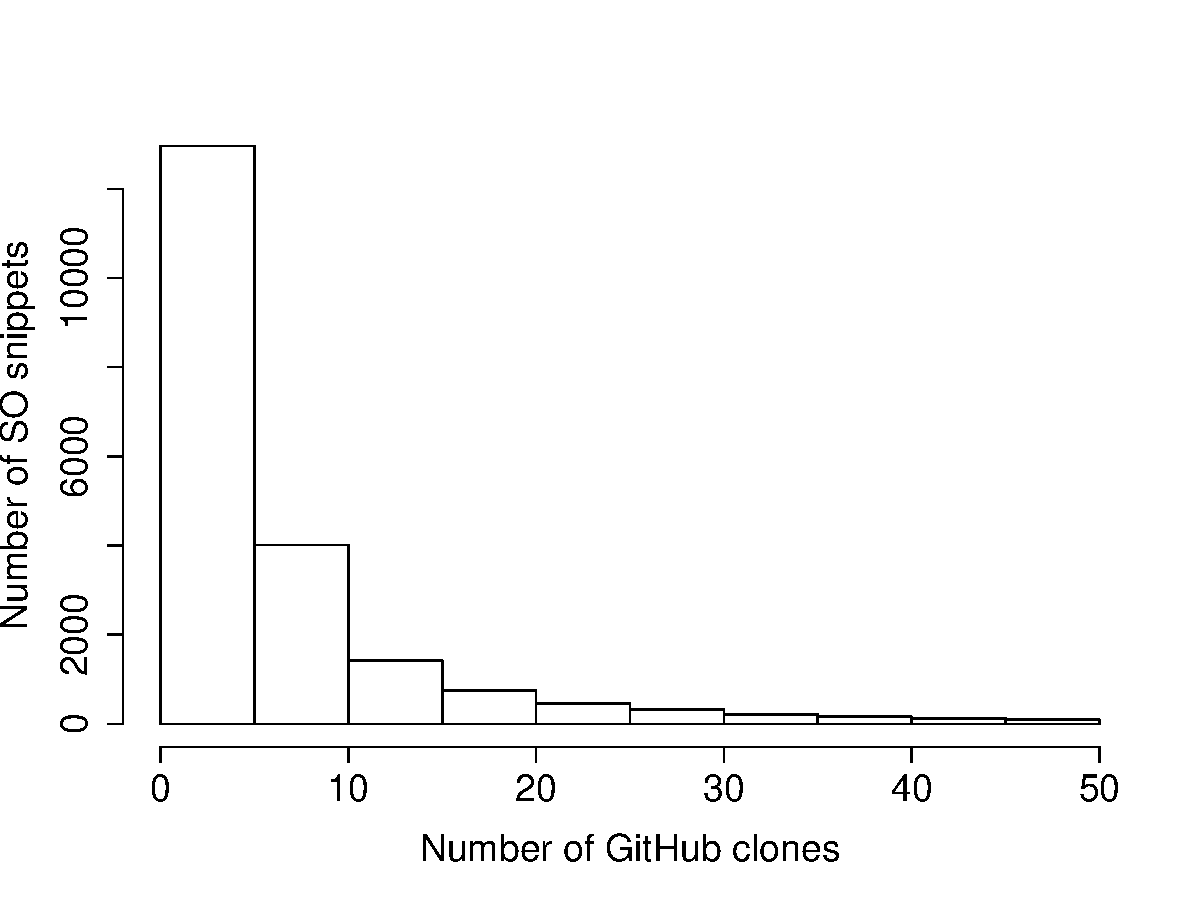
\includegraphics[scale=0.4]{figures/dist-gh-clone.pdf}
	\caption{Distribution of number of GitHub clones}
	\label{fig:num-clone}
\end{figure}

We collect the original GitHub files which contain these similar counterparts Then we extract all co-occurred methods from these GitHub files and treat them as candidate code fragments. For each candidate in each GitHub file, we cluster its similar counterparts from other files. We keep only the clusters with size of at least two and return the remaining clusters in descending order of size.

For 11,110 out of 21K SO queries, {\tool} can retrieve related code fragments from GitHub. That is, using our SO query code base and GitHub search code corpus, {\tool} can find common co-occurring code for 52.4\% of the queries. The SO queries have a median of 24 common co-occurring methods in GitHub and a mean of 74 common co-occurring methods. The retrieved methods have a median of 12 average lines of code, and a mean of 14 average lines of code. The distribution of number of related methods and distribution of average lines of code are shown in Figure \ref{fig:num-related} and \ref{fig:avg-loc} respectively.

From the figures we can see that a SO query most commonly have less than ten common co-occurring code fragments, and most of the SO queries have less than 50 common co-occurring methods in GitHub. Most related methods for a query will have five to thirty average lines of code.

\begin{figure}
	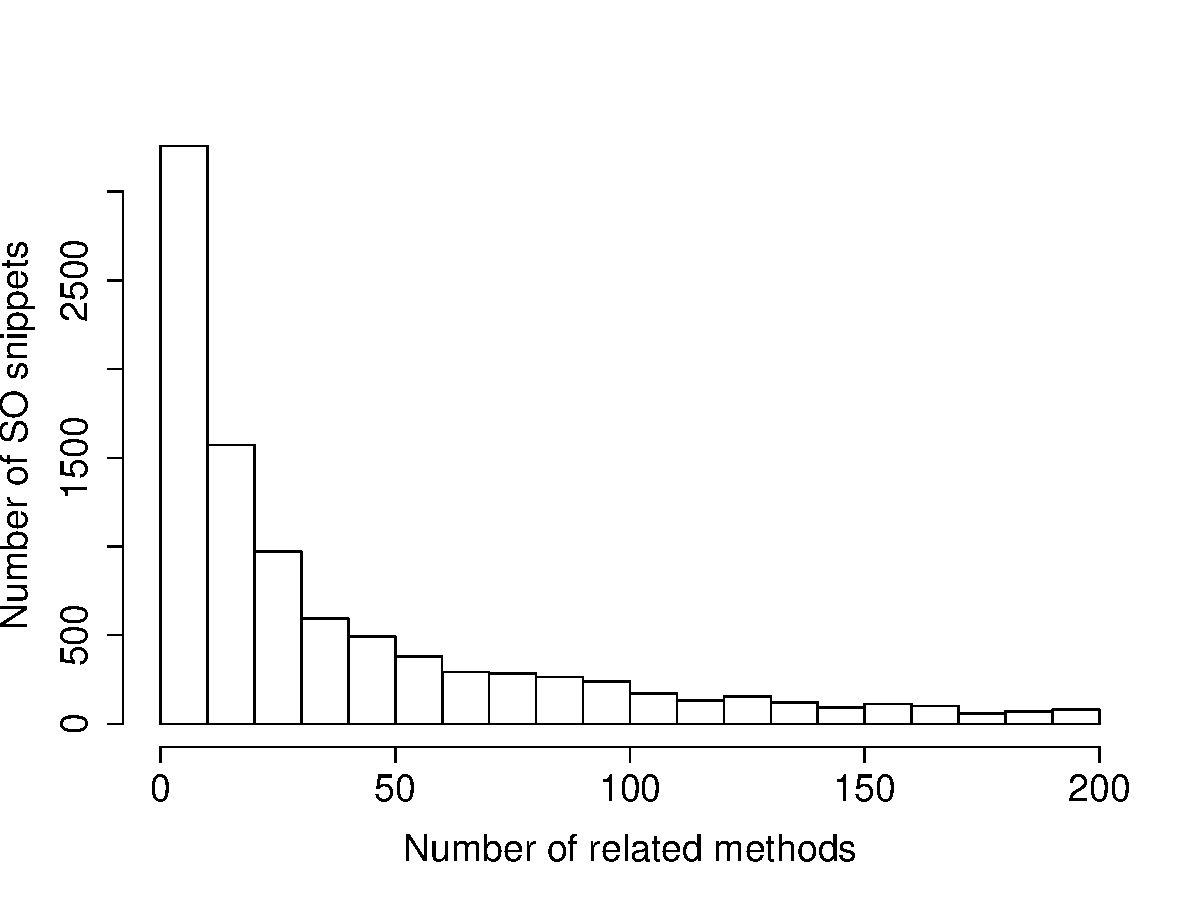
\includegraphics[scale=0.4]{figures/dist-related.pdf}
	\caption{Distribution of number of related methods}
	\label{fig:num-related}
\end{figure}

\begin{figure}
	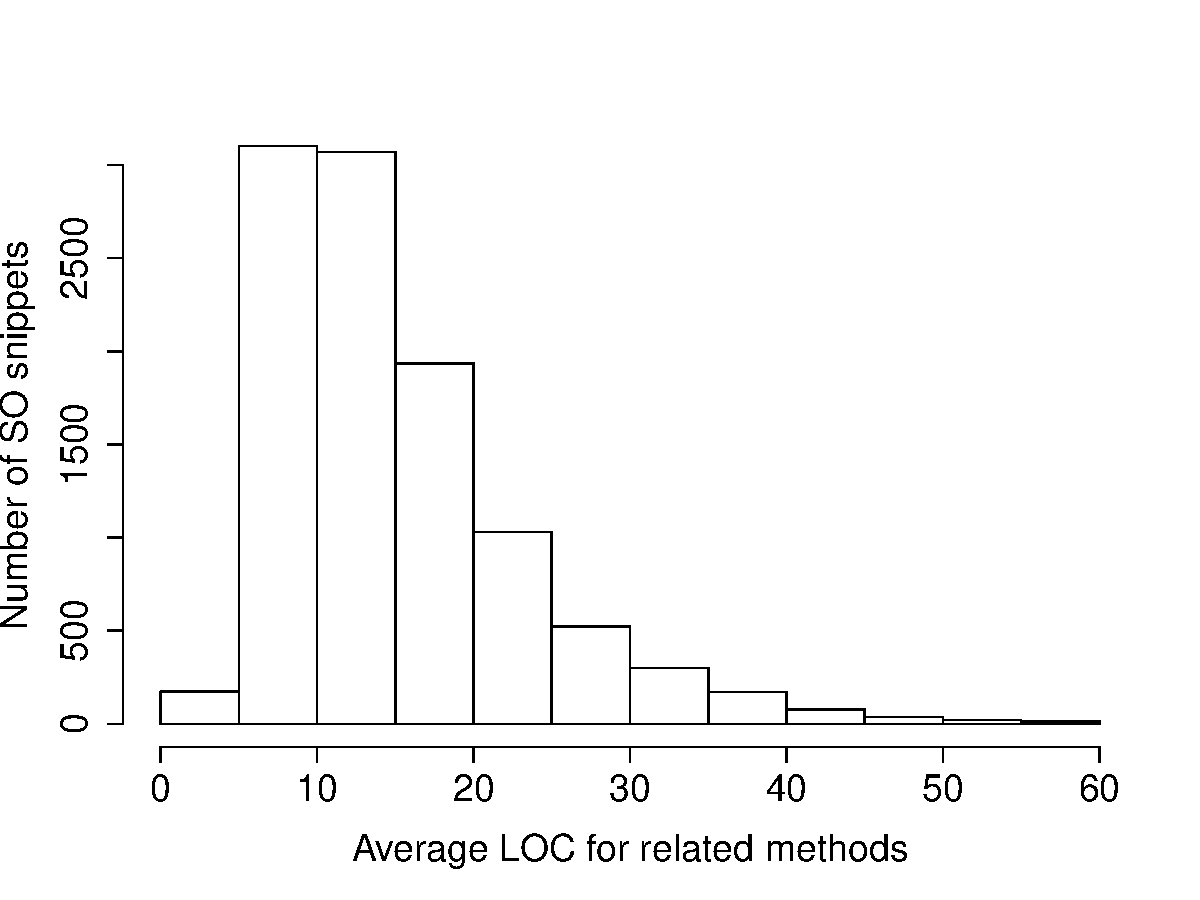
\includegraphics[scale=0.4]{figures/dist-loc.pdf}
	\caption{Distribution of average LOC of related methods}
	\label{fig:avg-loc}
\end{figure}




\subsection{Manual analysis and categorization}
We randomly select 30 SO snippets with its recommended related code fragments from the 11,110 groups, and manually examine whether the recommended code fragments are related to the SO input or not, and categorize why we call the relationship a relevant one.

We use $Precision@k$ metric to evaluate \tool\  which is defined as follows:
\begin{equation}
Precision@k = \frac{1}{N}\sum_{i=1}^{N}\tfrac{\left | relevant_{i,k} \right |}{k}
\end{equation}
where $\left | relevant_{i,k} \right |$ represents the number of positive related results in the top $k$ results for query $i$, $N$ is the number queries we evaluate, which is $30$. $k$ is the number of top results we examine, here we use $k=1$ and $k=3$.

\tool\ achieves 80\% and 75.6\% for $Precision@1$ and $Precision@3$ respectively. That is to say, for the 30 top 1 recommended results, 24 of them are manual examined as related, for the 90 top 3 recommended resutls, 68 of them are related.

We find the following types of relevance in our sample set:
\begin{itemize}
	\item A complementary method that adds more functionality
	\item A supplmentary method that helps with, or gets help, from the query 
	\item A different implementation for the query	
\end{itemize}

\begin{table}
	\begin{center}
		\begin{tabular}{ c|c|c } 
			Category & Top 1 & Top 3 \\\hline
			Complementary method &  12 & 33\\\hline 
			Supplementary method &  11 & 31 \\ \hline
			Different implementation &  1 & 4 \\ \hline
			Not related & 6 & 22
		\end{tabular}		
	\end{center}
	\caption{Categorization of related methods}
	\label{tab:categorization}
\end{table}
	
	

\subsubsection{Complementary method} In this category, the query code can function alone, but the recommended related method provides extra functionality to the query code and will further complete the user class. For the example shown as Listing ~\ref{lst:mot-query} and ~\ref{lst:mot-related} in Section~\ref{sec:intro}, The query snippet implements unzip a folder in Java.  \tool\ recommends {\ttt zip} function. These two methods can function independently, but often implemented together to get a stronger ability for file manipulation. Similarly, {\ttt decrypt} function for {\ttt encrypt} and {\ttt onPause} function for {\ttt onCreate}. The two methods do not have any direct function call association between them, but they complete each other with extra functionality and are often implemented together in real-life scenarios. 

\subsubsection{Supplementary method} The recommended related code serves as a helper function to the query, or vice versa. One may make function call to the other. For example the {\ttt merge} function for {\ttt sort}. {\ttt sort} calls {\ttt merge} as a helper function and cannot achieve functionality without it. Also in our second example Table ~\ref{tab:suppl-examples}, our recommended related code {\ttt loadDrawable} calls {\ttt queueJob} inside its method body. There is another related method being recommended together, which is shown below \ref{lst:part2}. This code is also called by {\ttt loadDrawable}, the related methods give the user a broader picture of the whole class,point to a higher level of functionality the user may want to implement, and also direct the user to the most-frequently used higher level functionality and its auxiliaries.
\begin{lstlisting}[caption={Recommended code \#2}, label={lst:part2}]
public static Drawable getDrawableFromCache(String url) {
	if (DrawableManager.cache.containsKey(url)) {
		return DrawableManager.cache.get(url);
	}
	
	return null;
}	
\end{lstlisting}

\subsubsection{Different implementation} This category represents those recommended related methods that have similar functionality to the query code. The recommended result provides an alternative, or a more detailed or extended implementation for the functionality. As shown in Table ~\ref{tab:diff-examples}, both of the methods implement sorting values in a {\ttt Map}, the query store the map entries in a {\ttt SortedSet}, while the recommended code uses {\ttt LinkedList}, and shows how to iterate a {\ttt Map}. For the {\ttt encrypt} function in Table ~\ref{tab:compl-examples}, \tool\ also recommended an alternative implementation with {\ttt String} inputs, as shown in Listing ~\ref{lst:encryt}.


\begin{lstlisting}[caption={different implementation for \texttt{encrypt}}, label={lst:encryt}]
public static String encrypt(final String password, String message) throws GeneralSecurityException {
	try {
		final SecretKeySpec key = generateKey(password);
		log("message", message);
		byte[] cipherText = encrypt(key, ivBytes, message.getBytes(CHARSET));
		//NO_WRAP is important as was getting \n at the end
		String encoded = String.valueOf(
			Base64.encodeToString(cipherText, Base64.NO_PADDING ));
		log("Base64.NO_WRAP", encoded);
		return encoded;
	} catch (UnsupportedEncodingException e) {
		if (DEBUG_LOG_ENABLED)
			Log.e(TAG, "UnsupportedEncodingException ", e);
		throw new GeneralSecurityException(e);
	}
}
\end{lstlisting}



\subsection{Comparison with code search engines}
In this experiment we compare the recommendation results of \tool\ with those from code search engines. We choose Google search engine since its the most popular destination when people look for programming assistance. We also compare to {\ttt FaCoY}~\cite{kim2018Facoy}, a code-to-code search engine which proved to have state-of-art precision. It uses SO snippets as its query base and indexes GitHub files as search space. {\ttt searchcode}~\cite{searchcode} and {\ttt Krugle}~\cite{krugle} are another two online code-to-code search engines. We only compare with {\ttt FaCoY} because it beats {\ttt searchcode} and {\ttt Krugle} in the total number of outputs and precision of outputs when using SO snippets as queries~\cite{kim2018Facoy}. 
We look for whether the search engines can also retrieve top 1 related code fragments recommended by \tool\ in their top 10 search results. 

For one out of the ten queries, {\ttt FaCoY} can return the related code recommended by \tool\ in its top 10 search results. This results from the related code being very similar to the query, as shown in Table ~\ref{tab:facoy-example}. For the rest of nine queries, the related code is not similar to the query, so it cannot be retrieved by {\ttt FaCoY}.

As for Google search engine, for five out of the ten queries, Google can locate the GitHub file(s) which contain similar methods to the query, therefore we can find the related code recommended by \tool\ inside these GitHub files. However, Google can only retrieve the full files, while \tool\ can point to the method which is mostly used among these files. 

By performing the comparison above, we can see that code search engines may not fulfill the purpose of recommending related code as \tool{}.


\lstset{
	frame=none,
	aboveskip=0pt,
	belowskip=0pt,
	basicstyle=\tiny\ttfamily,
}
\begin{table*}\scriptsize
	\caption{Related code which can be retrieved by FaCoY}
	\label{tab:facoy-example}
	
	\setlength{\tabcolsep}{0.01\textwidth}
	\begin{tabular}{@{}p{0.49\textwidth}p{0.49\textwidth}@{}}
		\toprule
		Query Code Snippet & Recommended Related Code \\
		\midrule


\begin{lstlisting}
public int readFramesChanel(short[] sampleBuffer, int offset, int numFramesToRead,int channel) throws IOException, WavFileException
{
	if (ioState != IOState.READING) throw new IOException("Cannot read from WavFile instance");

	for (int f=0 ; f<numFramesToRead ; f++)
	{
		if (frameCounter == numFrames) return f;

		for (int c=0 ; c<numChannels ; c++)
		{
			if(channel==c)
			{
				sampleBuffer[offset] = (short) readSample();
				offset ++;
			}
			else
				readSample();
		}

		frameCounter ++;
	}

	return numFramesToRead;
}
\end{lstlisting}
		
		&
\begin{lstlisting}
public int writeFrames(int[] sampleBuffer, final int offSetIn, int numFramesToWrite) throws IOException
{
	if (this.ioState != IOState.WRITING) throw new IOException("Cannot write to WavFile instance"); //$NON-NLS-1$
	int offSet = offSetIn;
	for (int f = 0; f < numFramesToWrite; f++)
	{
		if (this.frameCounter == this.numFrames) return f;

		for (int c = 0; c < this.numChannels; c++)
		{
			writeSample(sampleBuffer[offSet]);
			offSet++;
		}

		this.frameCounter++;
	}

	return numFramesToWrite;
}
		
\end{lstlisting}
\\

\bottomrule
	\end{tabular}
\end{table*}
		

